\documentclass[titlepage]{article}
\usepackage{minted}
\usepackage[margin=0.5in]{geometry}
\usepackage{graphicx}

\title{Internet Technologies Lab Report\\Assignment 1}
\author{Md Sahil\\BCSE IV\\Roll-001710501029}
\date{}

\begin{document}
    {\maketitle}

    \section{Problem Statement}
    Implement a TCP-based key-value store. 
	The server implements the key-value store and clients 
	make use of it. The server must accept clients’ connections 
	and serve their requests for ‘get’ and ‘put’ key value pairs. 
	All key-value pairs should be stored by the server only 
	in memory. Keys and values are strings. 
	The client accepts a variable no of command line arguments 
	where the first argument is the server hostname followed 
	by port no. It should be followed by any sequence 
	of\\ 
    ``~get $\langle$~key$\rangle$~''\\ 
    and/or\\ 
    ``~put $\langle$~key$\rangle$~$\langle$~value$\rangle$~''. 

    \begin{minted}{bash}
./client 192.168.124.5 5555 put city Kolkata put country India get country get city get Institute
India
Kolkata 
<blank> 
    \end{minted}

	The server should be running on a TCP port. The server should support multiple 
    clients and maintain their key-value stores separately.\\~\\
    Implement authorization so that only few clients having the role “manager” can 
    access other’s key-value stores. A user is assigned the “guest” role by default. 
    The server can upgrade a “guest” user to a “manager” user 

    \section{Design \& Implementation}
    The program is implemented using Java.
    The program is divided into two sections the \emph{Server} and the \emph{Client}.

    \begin{figure}[!ht]
        \centering
        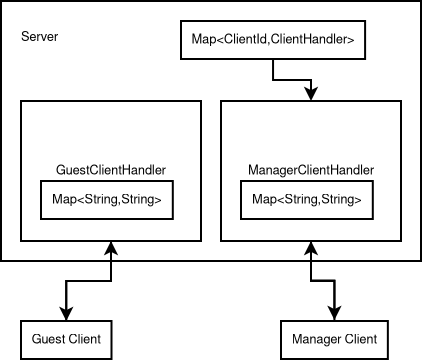
\includegraphics[scale=0.6]{./serverClient.png}
        \caption{Flow Diagram}
    \end{figure}

    \textbf{The Client} program has 2 threads running. The main thread runs the input console.
    The console takes input from the user and sends it to the server accordingly.

    \textbf{The Server} program has a main thread to run the console and a seperate thread for
    each client connected to it. The ClientHandler class ( implements the Runnable interface )
    handle the communication between the assigned client and the server. When multiple clients are
    connected multiple ClientHandler instances are generated. The ClientHandler instances also
    store the client data in a HashMap$\langle$String,String$\rangle$ data structure.

    The Port number of each client is treated as the ID for the client.
    Client data is stored in a HashMap as a member variable of the ClientHandler interface.

    The Server terminal can upgrade guest clients to managers or downgrade managers to guest.

    \pagebreak
    \section{Usage and Features}

    \subsection{Directory structure}
    The directory structure of the program is as follows:
    \begin{minted}{bash}
    .
    |-- Makefile
    |-- bin
    |   |-- client
    |   |   |-- Client$Listener.class
    |   |   |-- Client.class
    |   |   `-- Main.class
    |   `-- server
    |       |-- ClientHandler.class
    |       |-- GuestClientHandler.class
    |       |-- Main.class
    |       |-- ManagerClientHandler.class
    |       |-- Server$Terminal.class
    |       `-- Server.class
    |-- run.sh
    `-- src
        |-- client
        |   |-- Client.java
        |   `-- Main.java
        `-- server
            |-- ClientHandler.java
            |-- GuestClientHandler.java
            |-- Main.java
            |-- ManagerClientHandler.java
            `-- Server.java

    6 directories, 18 files
    \end{minted}

    \subsection{Compilation}
    In order to compile the program just run make while at the root directoy.
    \begin{minted}{bash}
        $ make
    \end{minted}

    To run the server use to following command.
    \begin{minted}{bash}
        $ java -cp bin/ server/Main <port>
    \end{minted}

    To run clients use the following command.
    The port number is the port in which the server runs.
    \begin{minted}{bash}
        $ java -cp bin/ client/Main <port>
    \end{minted}

    \subsection{Usage}
    \subsubsection{Server commands}
    \begin{itemize}
    \item List connected clients
    \begin{minted}{shell-session}
    # list
    \end{minted}
    \item Upgrade guest clients
    \begin{minted}{shell-session}
    # upgrade <client_port>
    \end{minted}
    \item Downgrade guest clients
    \begin{minted}{shell-session}
    # downgrade <client_port>
    \end{minted}
    \end{itemize}
    \subsubsection{Client commands}
    \begin{itemize}
    \item Put command
    \begin{minted}{shell-session}
    $ put <key> <value>
    \end{minted}
    \item Get command
    \begin{minted}{shell-session}
    $ get <key>
    \end{minted}
    \end{itemize}
    The get and put commands are concatinatable.
    \subsubsection{Manager commands}
    Along with all the client commands the manager also has
    some additional commands.
    All manager commands are accompanied by the prefix $mgr$.
    \begin{itemize}
    \item List connected clients
    \begin{minted}{shell-session}
    # mgr list
    \end{minted}
    \item Put or get command on client
    \begin{minted}{shell-session}
    # mgr <clienti_d> put <key> <value> get <key> ...
    \end{minted}
    \end{itemize}
    

    \subsection{Features}
    \begin{itemize}
    \item The program is an interative program. There are interative shells running on both
        server and client end points.
    \item Depending on the permissions of the terminal, the shell prompt changes.
        For manager clients and the server, the shell prompt is \textbf{\#}.
        For regular clients the shell prompt is \textbf{\$}.
    \item The program is multi-threaded. Multiple clients can stay connected to the server
        simultaneously.
    \item Multiple servers can be run on different ports on the machine.
        A client can be connected to a single server only.
    \end{itemize}

	\pagebreak
    \subsection{Sample I/O}

    \begin{itemize}
    \item Server I/O
        \begin{minted}{shell-session}
	Server started at :127.0.1.1
	# Connected to :/127.0.0.1:39328
	Connected to :/127.0.0.1:39330
	list
	Guest:39328
	Guest:39330
	39330: put city Kolkata
	39330: get city
	# upgrade 39328
	Upgrading 39328
	# Connected to :/127.0.0.1:39328
	39328: mgr lisg
	39328: mgr list
	39328: mgr 39330 get city
	#
        \end{minted}
    \item Client 1 I/O
        \begin{minted}{shell-session}
	Connection established with server!
	$ put city Kolkata
	$ get city
	Kolkata
	$
        \end{minted}
    \item Client 2 I/O
        \begin{minted}{shell-session}
	Connection established with server!
	upgrade
	# mgr lisg
	Invalid command
	# mgr list
	Manager:39328
	Guest:39330
	# mgr 39330 get city
	Kolkata
	#
        \end{minted}
    \end{itemize}


    


\end{document}
